\documentclass[conference]{IEEEtran}
\usepackage{times}

% numbers option provides compact numerical references in the text. 
\usepackage[numbers]{natbib}
\usepackage{multicol}
\usepackage[bookmarks=true]{hyperref}
\usepackage{amsmath}
\usepackage{amsthm}
\usepackage{amssymb}
\usepackage{graphicx}
\usepackage[table]{xcolor}
\usepackage{multirow}
\usepackage{color}  % For Highlighting
\usepackage[normalem]{ulem}
\usepackage{soul}
\usepackage[ruled]{algorithm2e}

% Editing tools
\newcounter{RamCount}
\newcounter{DavidCount}
\newcounter{BrentCount}
\newcommand{\hilight}[1]{\colorbox{yellow}{#1}}
\newcommand{\David}[1]{\textcolor{red}{\textbf{\theDavidCount}: (#1)} \addtocounter{DavidCount}{1}}
\newcommand{\Ram}[1]{\textcolor{blue}{\textbf{\theRamCount}: (#1)} \addtocounter{RamCount}{1}}
\newcommand{\Brent}[1]{\textcolor{brown}{\textbf{\theBrentCount}: (#1)} \addtocounter{BrentCount}{1}}
\newcommand{\Dan}[1]{\textcolor{magenta}{(#1)}}
\newcommand{\Audrey}[1]{\textcolor{maroon}{(#1)}}

%% Custom macros
\newcommand{\Real}{\mathbb{R}}
\newtheorem{defn}{Definition}
\newtheorem{ex}[defn]{Example}

\pdfinfo{
   /Author (Daniel Bruder)
   /Title  (Modeling and Control of Soft Robots using the Koopman Operator and Model Predictive Control)
   /CreationDate (D:20101201120000)
   /Subject (Robots)
   /Keywords (Soft Robots; Koopman Operator; Model Predictive Control)
}

\begin{document}

% paper title
\title{Modeling and Control of Soft Robots using the Koopman Operator and Model Predictive Control}

% You will get a Paper-ID when submitting a pdf file to the conference system
\author{Author Names Omitted for Anonymous Review. Paper-ID [add your ID here]}

%\author{\authorblockN{Daniel Bruder}
%\authorblockA{Department of Mechanical Engineering\\
%University of Michigan\\
%Ann Arbor, Michigan 48109\\
%Email: bruderd@umich.edu}
%\and
%\authorblockN{Homer Simpson}
%\authorblockA{Twentieth Century Fox\\
%Springfield, USA\\
%Email: homer@thesimpsons.com}
%\and
%\authorblockN{James Kirk\\ and Montgomery Scott}
%\authorblockA{Starfleet Academy\\
%San Francisco, California 96678-2391\\
%Telephone: (800) 555--1212\\
%Fax: (888) 555--1212}}


% avoiding spaces at the end of the author lines is not a problem with
% conference papers because we don't use \thanks or \IEEEmembership


% for over three affiliations, or if they all won't fit within the width
% of the page, use this alternative format:
% 
%\author{\authorblockN{Michael Shell\authorrefmark{1},
%Homer Simpson\authorrefmark{2},
%James Kirk\authorrefmark{3}, 
%Montgomery Scott\authorrefmark{3} and
%Eldon Tyrell\authorrefmark{4}}
%\authorblockA{\authorrefmark{1}School of Electrical and Computer Engineering\\
%Georgia Institute of Technology,
%Atlanta, Georgia 30332--0250\\ Email: mshell@ece.gatech.edu}
%\authorblockA{\authorrefmark{2}Twentieth Century Fox, Springfield, USA\\
%Email: homer@thesimpsons.com}
%\authorblockA{\authorrefmark{3}Starfleet Academy, San Francisco, California 96678-2391\\
%Telephone: (800) 555--1212, Fax: (888) 555--1212}
%\authorblockA{\authorrefmark{4}Tyrell Inc., 123 Replicant Street, Los Angeles, California 90210--4321}}


\maketitle

\begin{abstract}
%% Robots are hard to control
Controlling soft robots with precision is a challenge due in large part to the difficulty of constructing models that are amenable to model-based control design techniques.
%% Koopman operator their offers a solution
Koopman Operator Theory offers a way to construct explicit linear dynamical models of soft robots and to control them using established model-based linear control methods.
This method is data-driven, yet unlike other data-driven models such as neural networks, it yields an explicit control-oriented linear model rather than just a ``black-box'' input-output mapping.
%% Summary of contributions
This work describes this Koopman-based system identification method and its application to model predictive controller design.
%% Experiment and results
A model and MPC controller of a pneumatic soft robot arm was constructed via the method, and its performance was evaluated over several trajectory following tasks in the real-world. 
On all of the tasks, the Koopman-based MPC controller outperformed a benchmark MPC controller based on a linear state-space model of the same system.
\end{abstract}

\IEEEpeerreviewmaketitle

%% Insert all content here
\section{Introduction} 
\label{sec:intro}

%% Why soft robots?
%% Body softness has been shown to be useful for robots operating in unstructured/unpredictable environments, or alongside humans, but hard to control.
Soft robots have bodies made out of intrinsically soft and/or compliant materials.
This inherent softness enables them to safely interact with delicate objects, and to passively adapt their shape to unstructured environments \cite{rus2015design}.
Such traits are desirable for robotic applications that demand safe human-robot interaction such as wearable robots, in-home assistive robots, and medical robots.
Unfortunately, the soft bodies of these robots also impose modeling and control challenges, which have restricted their functionality to date. 
In fact, many novel soft devices such as soft grippers (cite), crawlers (cite), and swimmers (cite) exploit the flexibility of their bodies to achieve coarse behaviors such as grasping and locomotion, but do not exhibit precise control capabilities \Dan{don't forget to add citations here}.
% Emulating the functionality of the dexterous and precise soft systems found in nature such as octopus arms, elephant trunks, and tongues stems from the inherent difficulty of modeling continuum structures and controlling nonlinear dynamical systems.

% Unfortunately, their soft bodies also make soft robots notoriously difficult to model and control, limiting their functionality to date. 
% While their compliance enables such behavior it also makes soft robots challenging to model and control \cite{rus2015design}.

% Soft systems found in nature such as octopus arms, elephant trunks, and tongues display incredible dexterity and precision \cite{vogel2000cats}, but such functionality has yet to be realized in soft robots.
% Many novel devices such as soft grippers (cite), crawlers (cite), and swimmers (cite) exploit the flexibility of their bodies to achieve coarse behaviors such as grasping and locomotion, but do not exhibit precise control capabilities
% can be attributed to two innate characteristics of soft systems: continuum structure, and nonlinear dynamical behavior. 


%% Technical challenges to modeling: continuum structure
% Even building models for soft robots presents a challenge.
The challenge in constructing such precise control techniques is due in large part to the difficulty of devising models of soft robots that are amenable to model based control design techniques.
% Mathematical models are a convenient tool for predicting behavior and designing controllers for robots, but useful models are not as readily available for soft robots as for rigid-bodied ones \Ram{citation?}.
Consider for instance rigid-bodied robotic systems that are made up of rigid links connected together by discrete joints.
% Rigid-bodied robots consist of rigid links connected together by discrete joints.
%It has been shown that the full geometry of a rigid-bodied system can be described in terms of joint deformations, making joint deformations the canonical choice of state variables for rigid-bodied robots \cite{spong2008robot}.  %[Brent thinks the following would be a little easier to read:]
Since joint displacements can be used to fully describe the configuration of a rigid-bodied system, joint displacements and their derivatives make a natural choice for the state variables for rigid-bodied robots \cite{spong2008robot}.
One can use this choice of state variables to describe the dynamics of the rigid-bodied robot.
This, as a result, makes the application of model-based control design techniques such as feedback linearization \cite{}, nonlinear model predictive control \cite{}, LQR-trees \cite{}, sequential action control \cite{ansari2016sequential}, and others feasible. \Dan{don't forget to add citations here} 

Soft robots, in contrast, do not exhibit localized deformation at discrete joints, but instead deform continuously along their bodies and have infinite degrees-of-freedom.
In the absence of joints, there does not yet exist a canonical choice of state variables to describe the geometry of a soft robot.
% Instead, it is common practice to choose a state made up of observable parameters, such as end-effector position (cite our koopman paper), curvature of body (cite), or fluid pressure (cite) \Dan{think of better example(s)}.
As a result, existing representations are typically only rich enough to describe the system under restrictive simplifying assumptions.
For example, the popular piecewise constant curvature model \cite{webster2010design} provides a low-dimensional description of the shape of continuum robots, but only under the assumption that bending occurs in sections of constant curvature.
Other simplified models such as pseudo-rigid-body (cite) and quasi-static \cite{bruder2018iros} (cite others), have demonstrated sufficient accuracy for some objectives (cite), \Dan{don't forget to add citations here} 
but they are only able to describe the behavior in a subset of configurations of the soft robot which can make applying model-based control design techniques impractical. 

%% FIGURE: Overview of the different system representations and control approaches
\begin{figure}
    \centering
    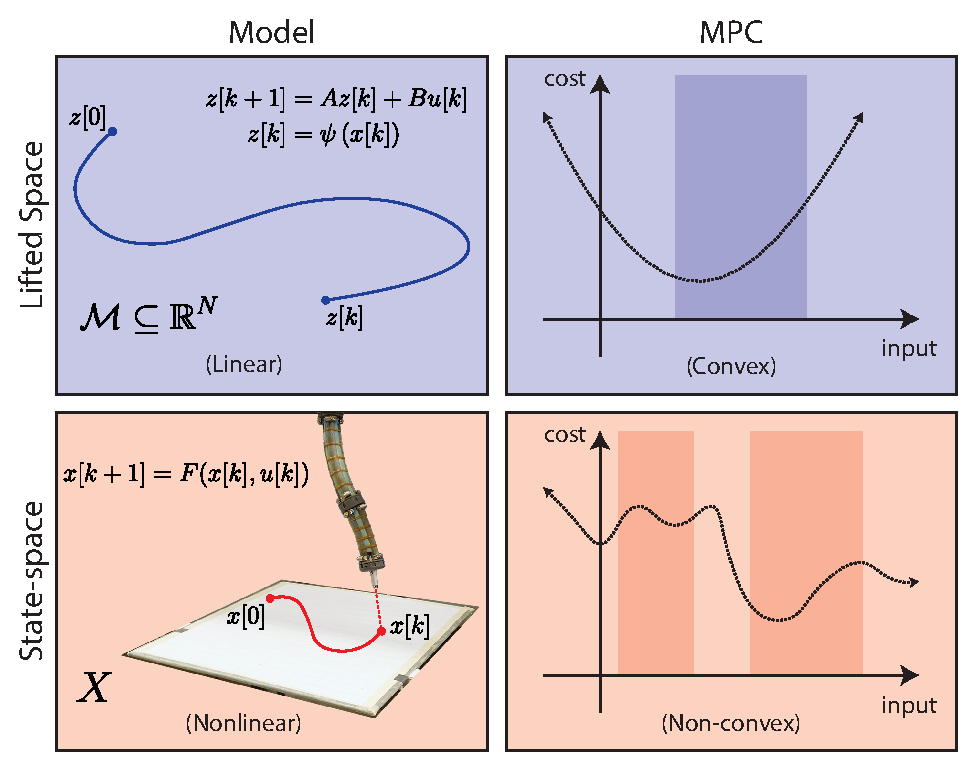
\includegraphics[width=\linewidth]{figures/overview_v8.pdf}
    \caption{A nonlinear dynamical system (bottom-left) has a \emph{linear} representation in the \emph{lifted} space made up of all real-valued functions (top-left). While a model predictive controller (MPC) designed for the nonlinear system in state-space requires solving a non-convex optimization problem to choose inputs at each time-step (bottom-right), this problem is convex for an MPC controller designed for the lifted linear system (top-right). This paper develops a data driven method to construct such a lifted model representation  for soft robotic systems in the presence of outliers and a convex, model-based control design technique for such systems. }
    \vspace*{-0.5cm}
    \label{fig:overview}
\end{figure}

%% data-driven models: don't make assumptions but not great for building controllers
% \Dan{This paragraph is a mess. Going to step away and come back to it}
Alternatively, data-driven methods, such as machine learning and neural networks, can be applied to construct models for soft robots without making structural simplifying assumptions.
Such models serve as a ``black-box'' by mapping from inputs to outputs and have been shown to predict behavior well across various configurations of the soft robot  \cite{gillespie2018learning, thuruthel2018model}.
However, since no explicit model is constructed, it can be challenging to apply existing model-based control design techniques.
% While such ``black-box'' models have been shown to predict behavior well, they offer little insight when it comes to controller design.
% \Ram{can you be more explicit here?} 

%% Technical challenge to control: Nonlinear dynamical behavior (think about this more and fix it)
% The inherently nonlinear dynamical behavior of soft robots presents a control challenge (CITE LASCHI CONTROL PAPER).
% Linear dynamical systems obey the \emph{superposition principle} (cite), which has enabled the development of powerful tools that render the task of controlling linear systems almost trivial.
% Unfortunately, the superposition principle does not hold for nonlinear dynamical systems and consequently there is no universal approach to controlling them.
% Numerical control techniques, such as nonlinear model predictive control (NMPC), have become popular due to ongoing increases in computational power and affordability.
% However, such methods require iteratively solving nonlinear non-convex optimization problems, for which global convergence is not guaranteed \cite{boyd2004convex}.
% which suffer from numerical issues such as suboptimal convergence and slow execution . 
% Numerical solvers may converge to suboptimal local extrema rather than optimal values.
% they are also slow...
% While this problem is not limited to soft robots (few mechanical systems exhibit completely linear dynamic behavior), soft robots are not as amenable to approximate linear descriptions as many other systems.

%% Koopman approach exists and can help here, it just needs some tweaks to work well for a real system
Koopman Operator Theory offers an approach that can overcome the challenges of modeling and controlling soft robots.
The Koopman operator approach is data-driven yet produces an explicit control-oriented model that is linear (though higher dimensional).
% Laid out in \citet{korda2018linear}, 
The approach leverages the linear structure of the Koopman operator to construct linear models of nonlinear controlled dynamical systems from input-output data \cite{bruder2018nonlinear, mauroy2016linear}, and to control them using established linear control methods \cite{Abraham-RSS-17, korda2018linear}.
In theory, this approach involves \emph{lifting} the state-space to an infinite-dimensional space of scalar functions (referred to as observables), where the flow of such observables along trajectories of the nonlinear dynamical system is described by the \emph{linear} Koopman operator.
In practice, however, it is not feasible to compute an infinite-dimensional operator, so a modified version of the Extended Dynamic Mode Decompostion (EDMD) is employed to compute a finite-dimensional projection of the Koopman operator onto a finite-dimensional subspace of all observables (scalar functions).
This approximation of the Koopman operator describes the evolution of the values of the output variables themselves, provided that they lie within the finite subspace of observables upon which the operator is projected.
Hence, this approach makes it possible to control the output of a nonlinear dynamical system using a linear controller designed for its linear Koopman representation.

%% Why this approach is uniquely well suited for soft robots: 
The Koopman approach to modeling and control is well suited for soft robots for several reasons.
Soft robots pose less of a physical threat to themselves or their surroundings when subjected to random control inputs than conventional rigid-bodied robots. 
This makes it possible to safely collect input-output data over a wide range of operating conditions, and to do so in an automated fashion. 
Furthermore, since the Koopman procedure is entirely data-driven, it inherently captures input-output behavior and avoids the ambiguity involved in choosing a discrete set of states for a structure with infinite degrees of freedom.
% Soft robots are also nonlinear dynamical systems, but this approach generates a linear system representation.
% As will be shown later, this linear representation can be used to construct a controller which computes control inputs by solving a convex optimization problem at each time step.

%% Our contribution: Modifications/additions needed to get this to reliably work for a real system
% This work applies the Koopman based system identification method from \citet{mauroy2016linear} and the Koopman based model predictive control method from \citet{korda2018linear} to a real soft robotic system.
The work presented here can be considered an extension of the work on Koopman-based modeling and control of \citet{mauroy2016linear} and \citet{korda2018linear}.
The novel contributions of this work, as depicted in Fig. \ref{fig:overview} are:
\begin{enumerate}
    \item An extension to the Koopman system identification procedure described in \cite{mauroy2016linear} to make the resulting Koopman operator both more sparse and less sensitive to outliers and noise in the training data,
    \item The application of this identified Koopman model for model predictive control of a physical soft robotic system.
\end{enumerate}
% We achieve (1) by introducing an $L^1$ penalty term into the least-squares optimization problem used to solve for the approximate Koopman operator.
Contribution (1) arose by necessity from the pursuit of contribution (2), since real mechanical systems suffer from both noise and computational limitations. \Dan{Rewrite this last sentence.} \Ram{my suggestion is that you highlight in the previous paragraph (the one about the utility of applying Koopman operator theory to soft robots) that pressure regulators for soft robots suck so they are super noisy which can make identifying such a Koopman model in practice difficult.}
% Data collected from physical mechanical systems is prone to noise, which can lead to over-fitting of data-driven models.
% Because real mechanical systems suffer from noise this step is 
% Both of these are desirable features when working with real systems, which suffer from noise and computational limitations.



%% Outline
The rest of this paper is organized as follows:
In Section \ref{sec:sysid} we formally introduce the Koopman operator and describe how it is used to construct linear models of nonlinear dynamical systems. 
In Section \ref{sec:mpc} we describe how the Koopman model can be used to construct a linear model predictive controller.
In Section \ref{sec:experiments} we describe the soft robot and the set of experiments used to evaluate the performance of a Koopman-based MPC controller.
In Section \ref{sec:conclusion} concluding remarks and perspectives are provided.





% %% Solution: Data-driven/linear representation, description of koopman approach
% In this paper, we present a novel method for the modeling and control of soft robots based on Koopman Operator Theory.
% This method addresses the challenges of modeling and control by offering a way to build a \emph{linear} model from data that still captures the \emph{nonlinear} input-output behavior of a soft robot.
% This approach is based on the system identification method originally presented in \citet{mauroy2017koopman} and the control approach laid out in \citet{korda2018linear}.
\section{Linear System Identification}
\label{sec:sysid}

%% Overview of this section
Any finite-dimensional, Lipschitz continuous nonlinear dynamical system has an equivalent infinite-dimensional linear representation in the space of all real-valued functions of the system's state \cite[Definition 3.3.1]{lasota2013chaos}.
This linear representation, which is called the Koopman operator, describes the flow of functions along trajectories of the system.
% The dual of the Koopman operator, the Perron-Frobenius operator, describes the dynamics of the system...
While it is not possible to numerically represent the infinite-dimensional Koopman operator, it is possible to represent its projection onto a finite-dimensional subspace as a matrix.
% Our goal is to construct models in this subspace in the form of a controlled linear dynamical system
% \begin{align}
%     \psi_{k+1} &= A \psi_{k} + B u_{k} \\
%     y_{k} &= C \psi_{k}
% \end{align}
% where $z$ is ... , $u$ is the input, and $y$ is the output of the system.
This section shows that for a given choice of basis functions, a \emph{lifted} linear dynamical system model can be extracted directly from the matrix approximation of the Koopman operator.
% As desired, system representations of this form lend themselves to linear control methods.
The remainder of this sections outlines the approach for constructing the Koopman operator approximation and the linear system representation from data.
Section \ref{sec:mpc} illustrates how this model can be incorporated into a model predictive control algorithm.

%% Overview of the Koopman operator and how it represents dynamical systems
\subsection{Koopman Representation of a Dynamical System}

%% System representation in state space
Consider a dynamical system
\begin{align}
    \dot{x}(t) &= F (x(t))
    \label{eq:nlsys}
\end{align}
where $x(t) \in X \subset \Real^n$ is the state of the system at time $t \geq 0$, $X$ is a compact subset, and ${F}$ is a continuously differentiable function.
Denote by $\phi(t,x_0)$ the solution to \eqref{eq:nlsys} at time $t$ when beginning with the initial condition $x_0$ at time $0$.
For simplicity, we denote this map, which is referred to as the \emph{flow map}, by $\phi_t (x_0)$ instead of $\phi (t, x_0)$.

%% System representation in the space of observables
The system can be lifted to an infinite dimensional function space $\mathcal{F}$ composed of all square-integrable real-valued functions with compact domain $X \subset \Real^n$.
Elements of $\mathcal{F}$ are called \emph{observables}.
In $\mathcal{F}$, the flow of the system is characterized by the set %semigroup 
of Koopman operators 
$U_t : \mathcal{F} \to \mathcal{F}$, for each $t \geq 0$,
which describes the evolution of the observables ${f \in \mathcal{F}}$ along the trajectories of the system according to the following definition:
\begin{align}
    U_t f = f \circ \phi_t,      
    % && \forall f \in \F, t \geq 0
    \label{eq:koopman}
\end{align}
where $\circ$ indicates function composition.
As desired, $U_t$ is a linear operator even if the system \eqref{eq:nlsys} is nonlinear, since for $f_1, f_2 \in \mathcal{F}$ and $\lambda_1, \lambda_2 \in \Real$
\begin{align}
    \begin{split}
    U_t (\lambda_1 f_1 + \lambda_2 f_2) &= \lambda_1 f_1 \circ \phi_t + \lambda_2 f_2 \circ \phi_t \\
    &= \lambda_1 U_t f_1 + \lambda_2 U_t f_2.
    \end{split}
\end{align}
Thus, the Koopman operator provides a linear representation of the flow of a nonlinear system in the infinite-dimensional space of observables (see Fig. \ref{fig:overview}) \cite{budivsic2012applied}.
Contrast this representation with the one generated by the (nonlinear) flow map that for each $t \geq 0$ describes how the initial condition evolves according to the dynamics of the system.
In particular if one wants to understand the evolution of an initial condition $x_0$ at time $t$ according to \eqref{eq:nlsys}, then one could solve the nonlinear differential equation to generate the flow map. 
On the other hand, one could apply $U_t$ (a linear operator) to the indicator function centered at $x_0$ (i.e. the function that is $1$ at $x_0$ and zero everywhere else) to generate an indicator function centered at the point $\phi_t(x_0)$.
% \Ram{you need to say something more explicit here. While $\phi$ describes how an initial condition flows according to the ODE, the Koopman operator describes how a function evolves according to the ODE. Notice that one can go back and forth between the representations...}.


%% Koopman-based system identification (consult ICRA paper)
\subsection{Identification of Koopman Operator}
\label{sec:koopid}

Since the Koopman operator is an infinite-dimensional object, it cannot be represented by a finite-dimensional matrix. 
Therefore, we settle for the projection of the Koopman operator onto a finite-dimensional subspace.
Using a modified version of the Extended Dynamic Mode Decomposition (EDMD) algorithm \cite{williams2015data} originally presented in \cite{mauroy2016linear,mauroy2017koopman}, we identify a finite-dimensional approximation of the Koopman operator via linear regression applied to observed data.

Define ${\bar{\mathcal{F}} \subset \mathcal{F}}$ to be the subspace of $\mathcal{F}$ spanned by ${N>n}$ linearly independent basis functions 
${ \{ \psi_i : \Real^n \to \Real \}_{i=1}^N}$.
We denote the image of $\psi_i$ as $ \mathcal{R}_i$ which is equal to ${ \{ w \in \Real | \exists x \in \Real^n \text{ such that } \psi_i(x) = w  \} }$.
For convenience, we assume that the first $n$ basis functions are defined as
\begin{align}
    &\psi_i(x) = x_i
    \label{eq:xinpsi}
\end{align}
where $x_i$ denotes the $i^{\text{th}}$ element of $x$.
Any observable $\bar{f} \in \bar{\mathcal{F}}$ can be expressed as a linear combination of elements of these basis functions
\begin{align}
    \bar{f} &= \theta_1 \psi_1 + \cdots + \theta_N \psi_N
    \label{eq:fexpanded}
\end{align}
where each $\theta_i \in \Real$.
To aid in presentation, we introduce the vector of coefficients ${\theta = [ \theta_1 \,  \cdots \, \theta_N ]^\top}$ and the \emph{lifting function} ${\psi : \Real^n \to \Real^N}$ defined as:
\begin{align}
    % \psi(x) &:= \begin{bmatrix} \psi_1 (x) & \cdots & \psi_N (x) \end{bmatrix}^\top.
    \psi(x) &:= \begin{bmatrix} x_i & \cdots & x_n & \psi_{n+1} (x) & \cdots & \psi_N (x) \end{bmatrix}^\top.
    \label{eq:lift}
\end{align}
We denote the image of $\psi$ as $\mathcal{M} = \mathcal{R}_1 \times \cdots \times \mathcal{R}_N \subset \Real^N$.
By \eqref{eq:fexpanded} and \eqref{eq:lift}, $\bar{f}$ evaluated at a point $x$ in the state space is given by
% Note that $\bar{\theta}$ provides a vector representation for ${ \bar{f} \in \bar{\mathcal{F}} }$, and $\bar{f}$ evaluated at a point $x$ is given by
% Then, $\bar{f} \in \bar{\mathcal{F}}$ can be expressed concisely as
\begin{align}
    \bar{f}(x) &= \theta^\top \psi (x)
    \label{eq:fvec}
\end{align}
We therefore refer to $\psi(x)$ as the \emph{lifted state}, and $\theta$ as the \emph{vector representation} of $\bar{f}$.

Given this vector representation for observables, a linear operator $L : \bar{\mathcal{F}} \to \bar{\mathcal{F}}$ can be represented as an ${N \times N}$ matrix. 
We denote by $\bar{U}_t \in \Real^{N \times N}$ the approximation of the Koopman operator in $\bar{\mathcal{F}}$, which operates on observables via matrix multiplication:
\begin{align}
    \bar{U}_t \theta = \theta'
\end{align}
where $\theta , \theta'$ are each vector representations of observables in $\bar{\mathcal{F}}$.
%% Pulled straight from ICRA paper below this line
Our goal is to find a $\bar{U}_t$ that describes the action of the infinite dimensional Koopman operator $U_t$ as accurately as possible in the $L^2$-norm sense on the finite dimensional subspace $\bar{\mathcal{F}}$ of all observables.

To perfectly mimic the action of $U_t$ on an observable ${\bar{f} \in \bar{\mathcal{F}} \subset \mathcal{F}}$, according to \eqref{eq:koopman} the following should be true for all  $x \in X$
\begin{align}
    \bar{U}_t \bar{f}(x) &= \bar{f} \circ \phi_t(x) \\
    ( \bar{U}_t {\theta} )^\top {\psi}(x) &=
    {\theta}^\top {\psi} \circ \phi_t(x) \\
    \bar{U}_t^\top \psi(x) &= {\psi} \circ \phi_t(x),
    \label{eq:UbarEq}
\end{align}
where the second equation follows by substituting \eqref{eq:fexpanded} and the last equation follows by cancelling $\theta^\top$.
Since this is a linear equation, it follows that for a given ${x \in X}$, solving \eqref{eq:UbarEq} for $\bar{U}_t$ yields the best approximation of $U_t$ on $\bar{\mathcal{F}}$ in the $L^2$-norm sense \cite{penrose1956best}:
\begin{align}
    \bar{U}_t = \left( {\psi}^\top(x) \right)^\dagger ( {\psi} \circ \phi_t(x) )^\top
    \label{eq:Uapprox}
\end{align}
where superscript $\dagger$ denotes the least-squares pseudoinverse.

%% How this is done on our system
To approximate the Koopman operator from a set of experimental data, we take $K$ discrete state measurements in the form of so-called ``snapshot pairs'' $(a[k] , b[k])$ for each $k \in \{1,\ldots,K\}$ where
% with sampling period $T_s$. We separate the data into a set of $K$ so-called ``snapshot pairs'' of the form ${ \{ a_k , b_k \} \in \Real^{n \times 2} }$ where
\begin{align}
    a[k] &= x[k] \\
    b[k] &= \phi_{T_s} (x[k]) + \sigma[k],
    \label{eq:ab}
\end{align}
where $\sigma[k]$ denotes measurement noise, $T_s$ is the sampling period which is assumed to be identical for all snapshot pairs, and $x[k]$ denotes the measured state corresponding to the $k^\text{th}$ measurement.
% \Ram{is this where we mention that these measurements do not have to correspond to the state of the system but rather the things we can observe?}
Note that consecutive snapshot pairs do not have to be generated by consecutive state measurements. 
% For our basis of $\bar{\mathcal{F}}$, we choose the basis of monomials of $x$ with total degree less than or equal to $w$, which implies ${N=(n+m+w)!/\left((n+m)!w!\right)}$ \cite[Section III]{mauroy2016linear}. 
We then lift all of the snapshot pairs according to \eqref{eq:lift} and compile them into the following ${K \times N}$ matrices:
\begin{align}
    &\Psi_a := \begin{bmatrix} {\psi}(a[1])^\top \\ \vdots \\  {\psi}(a[K])^\top \end{bmatrix}
    &&\Psi_b := \begin{bmatrix} {\psi}(b[1])^\top \\ \vdots \\  {\psi}(b[K])^\top \end{bmatrix}
    \label{eq:Psi}
\end{align}
$\bar{U}_{T_s}$ is chosen so that it yields the least-squares best fit to all of the observed data, which, following from \eqref{eq:Uapprox}, is given by 
\begin{align}
    \bar{U}_{T_s} &:= \Psi_a^\dagger \Psi_b.
\end{align}

%% Incorporating Delays
Sometimes a more accurate model can be attained by incorporating delays into the set of snapshot pairs. 
To incorporate these delays, we define the snapshot pairs as
\begin{align}
    a[k] &= \begin{bmatrix} x[k]^\top, & x[k-1]^\top & \ldots, & x[k-d]^\top \end{bmatrix}^\top \label{eq:snapd1} \\
    b[k] &= \begin{bmatrix} \left( \phi_{T_s} (x[k]) + \sigma_k \right)^\top & x[k]^\top & \ldots & x[k-d+1]^\top \end{bmatrix}^\top \label{eq:snapd2}
\end{align}
where $d$ is the number of delays.
We then modify the domain of the lifting function such that $\psi : \Real^{n+nd} \to \Real^{N}$ to accommodate the larger dimension of the snapshot pairs.
Once these snapshot pairs have been assembled, the model identification procedure is identical to the case without delays.
% without input delays or $\Real^{n+nd} \times \Real^{md}$ with input delays.

%% Koopman representation of controlled dynamical system
\subsection{Building Linear System from Koopman Operator}
%Brent: Building a Linear Model from the Koopman Operator
% I don't get the lack of articles in your section heading. 

For dynamical systems with inputs, we are interested in using the Koopman operator to construct discrete linear models of the following form
\begin{equation}
\begin{aligned}
    z[j+1] &= A z[j] + B u[j] \\
    x[j] &= C z[j]
    \label{eq:linSys}
\end{aligned}
\end{equation}
for each $j \in \mathbb{N}$, where $x[0]$ is the initial condition in state space, $z[0] = \psi(x[0])$ is the initial lifted state, $u[j] \in \Real^m$ is the input at the $j^{\text{th}}$ step, and $C$ acts as a projection operator from the lifted space onto the state-space.
Specifically, we desire a representation in which (non-lifted) inputs appear \emph{linearly}, because models of this form are amenable to real-time, convex optimization techniques for feedback control design, as we describe in Section \ref{sec:mpc}.

We construct a model of this form by first applying the system identification method of Section \ref{sec:koopid} to the following modified snapshot pairs
% \begin{align}
%     \alpha_k &= \begin{bmatrix} \psi(a_k)^\top & u_k^\top \end{bmatrix} \\
%     \beta_k &= \begin{bmatrix} \psi(b_k)^\top & u_k^\top \end{bmatrix} 
% \end{align}
\begin{align}
    &\alpha[k] = \begin{bmatrix} \psi(a[k]) \\ u[k] \end{bmatrix} 
    &&\beta[k] = \begin{bmatrix} \psi(b[k]) \\ u[k] \end{bmatrix}
    \label{eq:alpha}
\end{align}
for each $k \in \{1,\ldots,K\}$. 
The input $u[k]$ in snapshot $k$ is not lifted to ensure that it appears linearly in the resulting model.
With these pairs, we define the following ${K \times (N + m)}$ matrices:
\begin{align}
    &\Gamma_\alpha = \begin{bmatrix} \alpha[1]^\top \\ \vdots \\  \alpha[K]^\top \end{bmatrix}
    &&\Gamma_\beta = \begin{bmatrix} \beta[1]^\top \\ \vdots \\  \beta[K]^\top \end{bmatrix}
    \label{eq:Gamma}
\end{align}
and solve for the corresponding Koopman operator according to \eqref{eq:Uapprox}
\begin{align}
    \bar{U}_{T_s} &:= \Gamma_{\alpha}^\dagger \Gamma_\beta.
    \label{eq:koopGamma}
\end{align}
Note that by \eqref{eq:UbarEq} and \eqref{eq:koopGamma} the transpose of this Koopman matrix is the best approximation of a transition matrix between the elements of snapshot pairs in the $L^2$-norm sense \
\begin{align}
    \bar{U}_{T_s}^\top 
    \begin{bmatrix} \psi(a[k]) \\ u[k] \end{bmatrix} &\approx
    \begin{bmatrix} \psi(b[k]) \\ u[k] \end{bmatrix},
\end{align}
and we desire the best $A,B$ matrices such that
\begin{align}
    A \psi(a[k]) + B u[k] &\approx \psi(b[k])
    \label{eq:linSys_psi}
\end{align}
Therefore, the best $A$ and $B$ matrices of \eqref{eq:linSys} are embedded in $\bar{U}_{T_s}^\top$ and can be isolated by partitioning it as follows:
\begin{align}
    \bar{U}_{T_s}^\top &= 
    \begin{bmatrix} 
        A_{N \times N} &
        B_{N \times m} \\
        O_{m \times N} &
        I_{m \times m}
    \end{bmatrix}
    \label{eq:AB}
\end{align}
where $I$ denotes an identity matrix, $O$ denotes a zero matrix, and the subscripts denote the dimensions of each matrix.
The $C$ matrix is defined
\begin{align}
    C &= \begin{bmatrix} I_{n \times n} & O_{n \times (N-n)} \end{bmatrix}
    \label{eq:C}
\end{align}
since by \eqref{eq:xinpsi}, ${x = [ \psi_1(x) , \dots , \psi_n(x) ]}$.
Note we can also incorporate input delays into the model by appending them to the snapshot pairs as we did in \eqref{eq:snapd1} and \eqref{eq:snapd2}.


% \begin{align}
%     z_{k+1} &= A z_k + B u_k
%     \label{eq:linSys}
% \end{align}

% \begin{align}
%     \begin{bmatrix} \psi(b_k) \\ u_k \end{bmatrix} &=
%     \begin{bmatrix} A_{N \times N} & B_{N \times m} \\ O_{m \times N} & I_{m \times m} \end{bmatrix} 
%     \begin{bmatrix} \psi(a_k) \\ u_k \end{bmatrix}
% \end{align}


%% Why should we use lasso instead of the least-squares solution
\subsection{Practical Considerations: Overfitting and Sparsity} \label{subsec:sparsity}


%% FIGURE: Lifting and Projecting
\begin{figure}
    \centering
    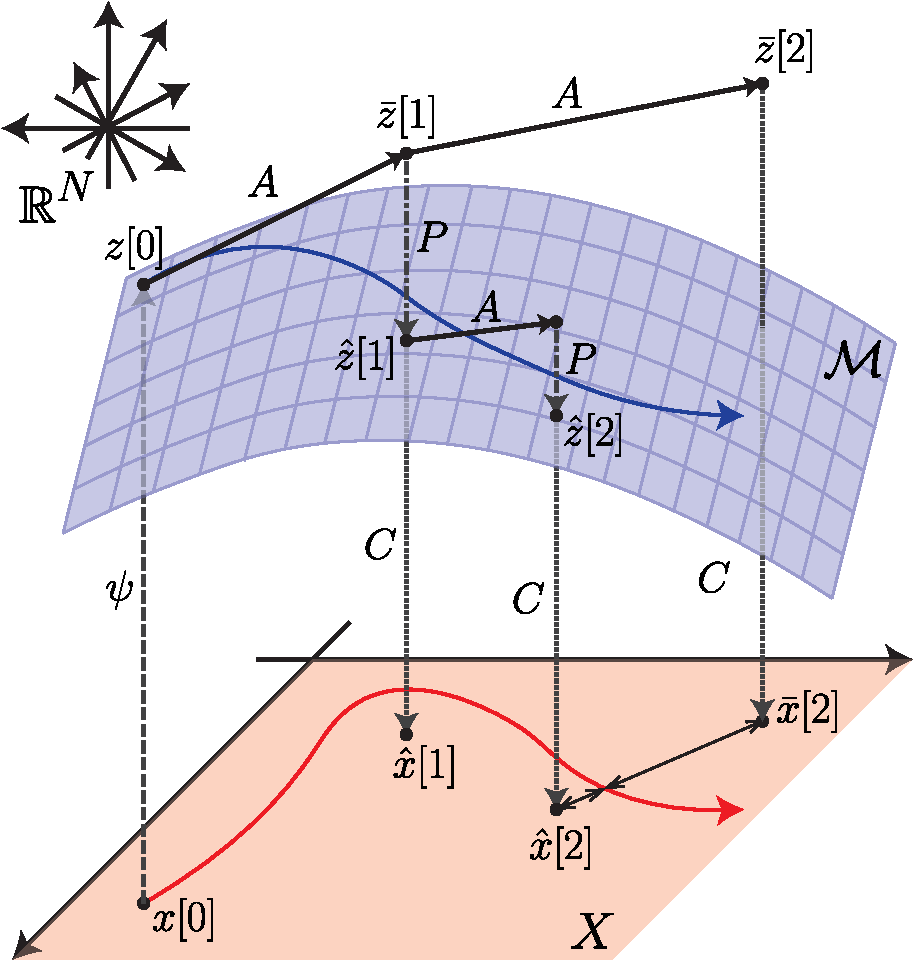
\includegraphics[width=0.8\linewidth]{figures/liftingManifold_v17.pdf}
    \caption{An illustration of the effect of deviating from the image of the lifted functions ${\cal M}$ and how it can be remedied by defining a projection operation as described in Section \ref{subsec:sparsity}. 
    The evolution of the finite dimensional system in the state space $X$ from $x_0$ is depicted as a red curve. 
    The lifted version of this evolution is depicted as the blue curve which is contained in $\cal{M}$.
    The discrete time system representation in the higher-dimensional space created by iteratively applying the state matrix $A$ to $z[j]$ may generate a solution that is outside of ${\cal M}$.
    Though one can still apply $C$ to $\bar{z}$ to project it back to $X$, this may result in poor performance.
    Instead, by projecting $\bar{z}[j]$ onto the manifold at each discrete time step to define a new lifted state $\hat{z}[j]$, the deviation from $\cal{M}$ is reduced, which improves overall predictive performance. }
    \label{fig:manifold}
    % \vspace*{-0.5cm}
\end{figure}

%% Need a way to deal with outliers
A pitfall of data-driven modeling approaches is the tendency to overfit.
While least-squares regression yields a solution that minimizes the total $L^2$ error with respect to the training data, this solution can be particularly susceptible to outliers and noise \cite{rousseeuw2005robust}.
To guard against overfitting to noise while identifying $\bar{U}_{T_s}$, we utilize the $L^1$-regularization method of Least Absolute Shrinkage and Selection Operator (LASSO) \cite{tibshirani1996regression}:
%% Lasso optimization problem
\begin{equation}
\begin{aligned}
\hat{\vec{U}}_{T_s} &= 
& \text{arg}~\underset{ \vec{U}_{T_s} }{\text{min}}
& & || \vec{\Gamma}_\alpha \vec{U}_{T_s} - \vec{\Gamma}_\beta ||_2^2 + \lambda || \vec{U}_{T_s} ||_1
\label{eq:lasso}
\end{aligned}
\end{equation}
where $\lambda \in \Real^{+}$ is the weight of the $L^1$ penalty term, and $\vec{\cdot}$ denotes a vectorized version of each matrix with dimensions consistent with the stated problem.
For $\lambda = 0$, \eqref{eq:lasso} provides the same unique least-squares solution as \eqref{eq:koopGamma}; as $\lambda$ increases it drives the elements of $\vec{U}_{T_s}$ to zero.
For an overview of the LASSO method and its implementation see \citet{tibshirani1996regression}.

%% Lasso promotes sparsity
The benefit of using $L^1$-regularization to reduce overfitting rather than $L^2$-regularization (e.g. ridge regression) is its ability to drive elements to zero, rather than just making them small.
This promotes sparsity in the resulting Koopman operator matrix (and consequently the $A$ and $B$ matrices).
Sparsity is desirable since it reduces the memory needed to store these matrices on a computer, enabling a higher dimensional set of basis functions to be used to construct the lifting function $\psi$.
% Sparsity is a desirable trait since it reduces the computational cost of solving the optimization problems involved in model predictive control. 
% As a consequence, control inputs can be calculated faster for models with sparser matrix representations, enabling higher bandwidth control.

%% The cost of sparsity, falling off the manifold
Though sparsity is desirable, it can come at the loss of accuracy in prediction. 
As illustrated in Fig. \ref{fig:manifold}, the lifting function $\psi$ maps from $\Real^n$ to $\mathcal{M}$, but at some time step $j$, $A\psi(a[j]) + B u[j]$ may not map onto $\mathcal{M}$.
When this happens and we try to simulate our linear model from an initial condition, it may leave the space of legitimate ``lifted states'' rapidly and fail to predict behavior accurately.
We therefore desire the sparsest model that minimizes the distance from $\mathcal{M}$ at each iteration.

This can be accomplished by applying a projection operator at each time step.
For each snapshot pair, the ideal projection operator $P$ should satisfy the following for all $k$
\begin{align}
    P \left( A {\psi}(a[k]) + B u[k] \right) &= \psi(b[k]).
\end{align}
To build an approximation to this operator, we construct the following $K \times N$ matrix,
\begin{align}
    &\Omega_a := \begin{bmatrix} \left( A {\psi}(a[1]) + B u[1] \right)^\top \\ \vdots \\  \left( A {\psi}(a[K]) + B u[K] \right)^\top \end{bmatrix}.
    \label{eq:Omega}
\end{align}
Then the best projection operator in the $L^2$-norm sense based on our data is given by
\begin{align}
    P := \left( \Omega_{a}^\dagger \Psi_b \right)^\top.
    \label{eq:P}
\end{align}
Composing $P$ with the $A$ and $B$ matrices in \eqref{eq:linSys} yields a modified linear model that significantly reduces the distance from $\mathcal{M}$ at each iteration,
\begin{align}
    z[j+1] &= \hat{A} z[j] + \hat{B} u[j]
    \label{eq:linSys_wP}
\end{align}
where $\hat{A} := PA$ and  $\hat{B} := PB$.
Algorithm \ref{alg:id} summarizes the proposed model construction process.


%% Sysid algorithm
\begin{algorithm}[t]
\SetAlgoLined
\KwIn{ $\lambda$ , $\{ a[k] , b[k] \}$ and ${ u[k] }$ for $k = 1 , ... , K$}
\textbf{Step 1:} Lift data via \eqref{eq:lift} \\
\textbf{Step 2:} Combine lifted data and inputs via \eqref{eq:alpha} \\
\textbf{Step 3:} Approximate Koopman operator $\bar{U}_{T_s}$ via \eqref{eq:lasso} \\
\textbf{Step 4:} Extract model matrices $A,B$ via \eqref{eq:AB} \\
\textbf{Step 5:} Identify projection operator $P$ via \eqref{eq:P} \\
\KwOut{$\hat{A} := PA$, $\hat{B} := PB$   }
 \caption{Koopman Linear System Identification}
 \label{alg:id}
\end{algorithm}
\section{Model Predictive Control}
\label{sec:mpc}

A system model enables the design of model-based controllers that leverage model predictions to choose suitable control inputs for a given task.
In particular, model-based controllers can anticipate future events, allowing them to optimally choose control inputs over a finite time horizon.
The most popular model-based control design technique is model predictive control (MPC), wherein one optimizes the control input over a finite time horizon, applies that input for a single timestep, and then optimizes again, repeatedly \cite{rawlings2009model}.
Applying MPC to design a controller for linear systems corresponds to solving a convex quadratic program. 

% optimizing the control input over an $N_h$ step planning horizon consists of solving a convex quadratic program.

Importantly, this is also the case during Koopman based MPC control design, wherein one solves the following program at each time instance $k$ of the closed-loop operation:
%% Linear MPC optimization problem
\begin{equation}
\begin{aligned}
& \underset{u[i] , z[i]}{\text{min}}
& & z[N_h]^{T} G_{N_h} z[N_h] + g_{N_h}^T z[N_h] + \cdots \\
&&& \sum_{i=0}^{N_h - 1} z[i]^T G_i z[i] + u[i]^T H_i u[i] + g_i^T z[i] + h_i^T u[i]\\
& \text{s.t.}
& & z[i+1] = \hat{A} z[i] + \hat{B} u[i] , \quad \forall i \in \{ 0 , \ldots , N_h - 1 \} \\
&&& E_i z[i] + F_i u[i] \leq b_i , \quad \forall i \in \{ 0 , \ldots , N_h - 1\} \\
&&& z[0] = \psi (x[k])
\end{aligned} \label{eq:mpc}
\end{equation}
where $G_i \in \Real^{N \times N}$ and $H_i \in \Real^{m \times m}$ are positive semidefinite matrices and where each time the program is called, the predictions are initialized from the current lifted state $\psi (x[k])$.
The matrices $E_i \in \Real^{c \times N}$ and $F_i \in \Real^{c \times m}$ and the vector $b_i \in \Real^{c}$ define state and input polyhedral constraints where $c$ denotes the number of imposed constraints.
Algorithm \ref{alg:mpc} summarizes the closed-loop operation of this Koopman based MPC controller.

%% MPC algorithm
\begin{algorithm}[t]
\SetAlgoLined
\KwIn{ Prediction horizon: $N_h$ \\
       \hspace{32pt} Cost matrices: $G_i , H_i , g_i , h_i$ for  $i = 0 , ... ,N_h$ \\
       \hspace{32pt} Constraint matrices: $E_i , F_i , b_i$ for $i = 0 , ... ,N_h$ \\
       \hspace{32pt} Model matrices: $\hat{A} , \hat{B}$ }
\For{ $k = 0 , 1 , 2 , ... $}{
\textbf{Step 1:} Set $z[0] = \psi ( x[k] )$ \\
\textbf{Step 2:} Solve \eqref{eq:mpc} to find optimal input $(u[i]^*)_{i=0}^{N_h}$ \\
\textbf{Step 3:} Set $u[k] = u[0]^*$ \\
\textbf{Step 4:} Apply $u[k]$ to the system
}
 \caption{Koopman-Based MPC}
 \label{alg:mpc}
\end{algorithm}


% \begin{equation}
% \begin{aligned}
%     J () &=
%     & & z_{N_p}^{T} P z_{N_p} + \cdots \\
%     &&& \cdots + \sum_{i=0}^{N_p - 1} z_i^T Q z_i + u_i^T R u_i + q^T z_i + r^T u_i\\
% \end{aligned} \label{eq:mpccost}
% \end{equation}

Since this optimization problem is convex, it has a unique globally optimal solution that can efficiently constructed without initialization \cite{boyd2004convex} for models with thousands of states and inputs  \cite{paulson2014fast,stellato2018osqp}.
This contrasts sharply with the MPC formulation for nonlinear systems (referred to as nonlinear model predictive control or NMPC \cite{allgower2012nonlinear}).
NMPC requires solving an optimization problem with nonlinear constraints and (potentially) nonlinear cost function.
As a result algorithms to solve such problems typically require initialization and can struggle to find globally optimal solutions \cite{polak2012optimization}.
Though techniques have been proposed to improve the speed of algorithms to solve NMPC problems \cite{patterson2014gpops,hereid2017frost} or even globally solve such problems without requiring initialization \cite{zhao2017control}, these formulations still take several seconds per iteration, which makes them too slow to be applied during real-time control.


% \subsubsection{Nonlinear MPC}
% %% Nonlinear MPC optimization problem
% \begin{equation}
% \begin{aligned}
% & \underset{u_{i} , x_{i}}{\text{min}}
% & & z_{N_p}^{T} P z_{N_p} + \sum_{i=0}^{N_p - 1} z_i^T Q z_i + u_i^T R u_i + q^T z_i + r^T u_i\\
% & \text{s.t.}
% & & z_{i+1} = f( z_i , u_i ) , \; i = 0 , \ldots , N_p - 1 \\
% &&& E z_i + F u_i \leq b , \; i = 0 , \ldots , N_p - 1 \\
% &&& z_0 = \psi(x_k).
% \end{aligned}
% \end{equation
\section{Experiments}
\label{sec:experiments}

%% Introduction
This section describes the robot and the set of experiments used to demonstrate the efficacy of the modeling and control methods from Sections \ref{sec:sysid} and \ref{sec:mpc}.
\Ram{you need to highlight the video which you will submit with the supplementary material here.}\Dan{How do I refer to the video? Do I just say 'the supplementary video submission' or should we have a link to youtube?}  \Brent{ I think just: ``see supplementary video file''.  I think you could expand this outline just a little to help the reader anticipate what's coming.  Perhaps say that in the following you will compare the performance of the nonlinear Koopman operator based MPC controller and a linear MPC controller. }

%% SUBS: Description of the system being 
\subsection{Robot Description: Soft Arm with Laser Pointer}
\label{sec:robot}

The robot used for the experiments is a suspended soft arm with a laser pointer attached to the end effector (see Fig. \ref{fig:rig}). 
The laser dot is projected onto a ${40\text{ cm} \times 40\text{ cm}}$ flat board which sits $30\text{cm}$ beneath the tip of the laser pointer when the robot is in its relaxed position (i.e. hanging straight down) \Dan{these numbers are made up need to measure}.
The position of the laser dot is measured by a digital webcam overlooking (aimed at) the board.

The arm itself consists of two sections that are each composed of three pneumatic artificial muscles or PAMs (also known as McKibben actuators \cite{tondu2012modelling}) adhered to a central foam spine by latex rubber bands (see Fig. \ref{fig:rig}).
The PAMs in the upper and lower sections are internally connected so that only three input pressure lines are required, and
they are arranged such that for any bending of the upper section, bending in the opposite direction occurs in the bottom section.
This ensures that the laser pointer mounted to the end effector points approximately vertically downward so that the light strikes the board at all times.
The pressures inside the actuators are regulated by three Enfield TR-010-g10-s pneumatic pressure regulators, which accept ${0-10}$V command signals corresponding to pressures of ${ \approx 0 - 140 }$ kPa.
In all the experiments there are three inputs corresponding to the voltages into the pressure regulators and a two dimensional state corresponding to the position of the laser dot with respect to the center of the board.

%% Rig figure
\begin{figure}
    \centering
    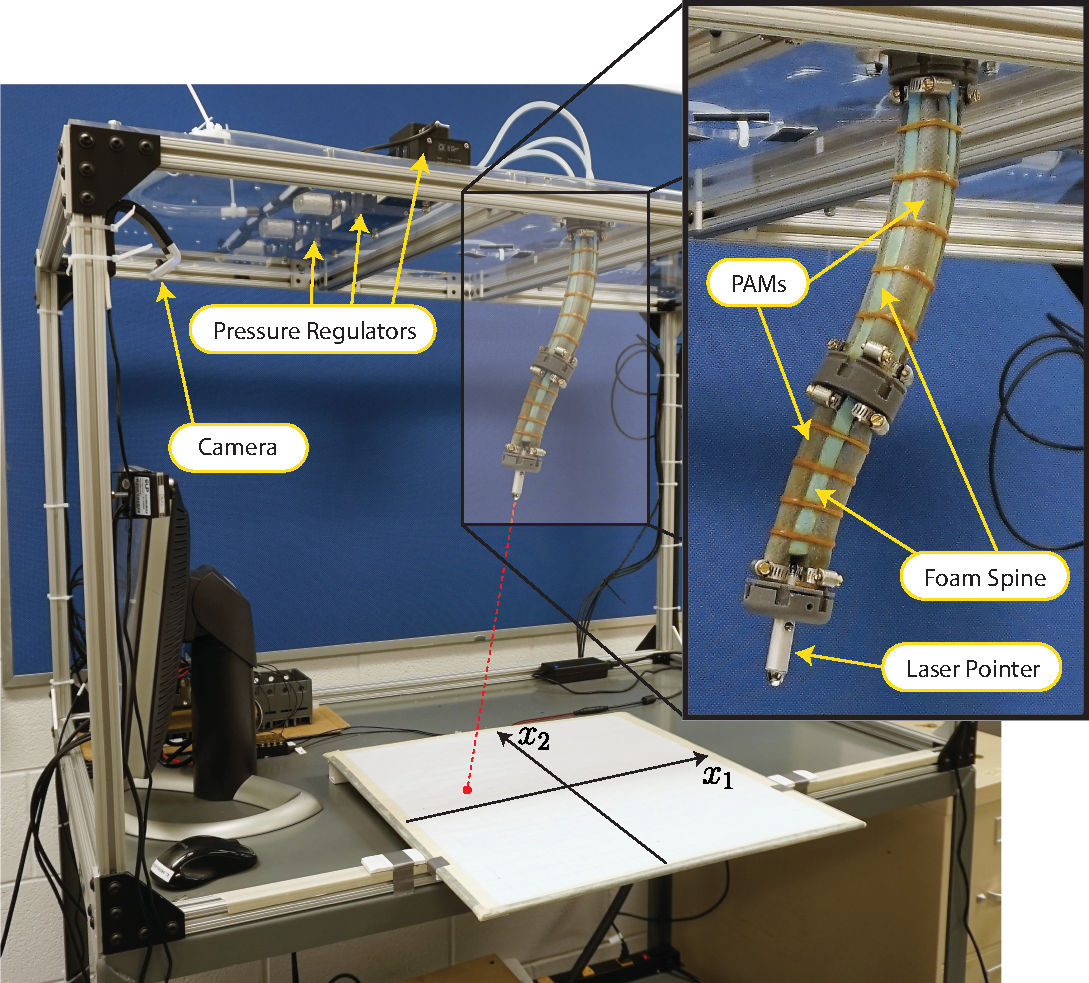
\includegraphics[width=\linewidth]{figures/rig_N_robot_smaller.pdf}
    \caption{The soft robot consists of two bending segments with a laser pointer attached to the end effector. A set of three pressure regulators is used to control the pressure inside of the pneumatic actuators (PAMs), and a camera is used to track the position of the laser dot.}
    \label{fig:rig}
    \vspace*{-0.5cm}
\end{figure}

%% SUBS: NOISE CHARACTERIZATION
\subsection{Characterization of Stochastic Behavior}
\label{sec:noise}

% An input-output system is said to exhibit \emph{stochastic} behavior if identical inputs sometimes produce different outputs.
Most mechanical systems demonstrate stochastic behavior (i.e. when an identical input under the same state produces a different output) to some extent.
Stochastic behavior is particularly problematic for pressure regulators \Ram{include a reference}, which can limit the precision of soft robotic systems that are attempting to perform dynamic tasks.
This can restrict the predictive capability of any model of our system.

We quantified the stochastic behavior of our soft robot system by observing the variations in output from period-to-period under sinusoidal inputs to the three actuators of the form
\begin{align} 
    u_k &= \begin{bmatrix} 6 \sin ( \frac{2 \pi}{T} k T_s ) + 3 \vspace{5pt} \\ 
    6 \sin ( \frac{2 \pi}{T} k T_s - \frac{T}{3} ) + 3 \vspace{5pt} \\ 
    6 \sin ( \frac{2 \pi}{T} k T_s  - \frac{2T}{3}) + 3\end{bmatrix}
    \label{eq:unoise}
\end{align}
for periods of $T = 6,7,8,9,10,11,12$ seconds and a sampling time of $T_s = 0.1$ seconds with a zero-order-hold between samples. 
Under these inputs, the laser dot traces out a circle, with some variability in the trajectory over each period.
In Fig.~\ref{fig:noise} the trajectories over 210 periods are superimposed along with the average over all trials.
Nearly all of the observed points fell within 1 cm of the mean trajectory.
Given this inherent stochasticity of our soft robotic system, even the best controller may only be able to control the output to within 1 cm of the desired trajectory.
\Dan{Still needs rewording}.

%% FIG: Noise inherent to the system
\begin{figure}
    \centering
    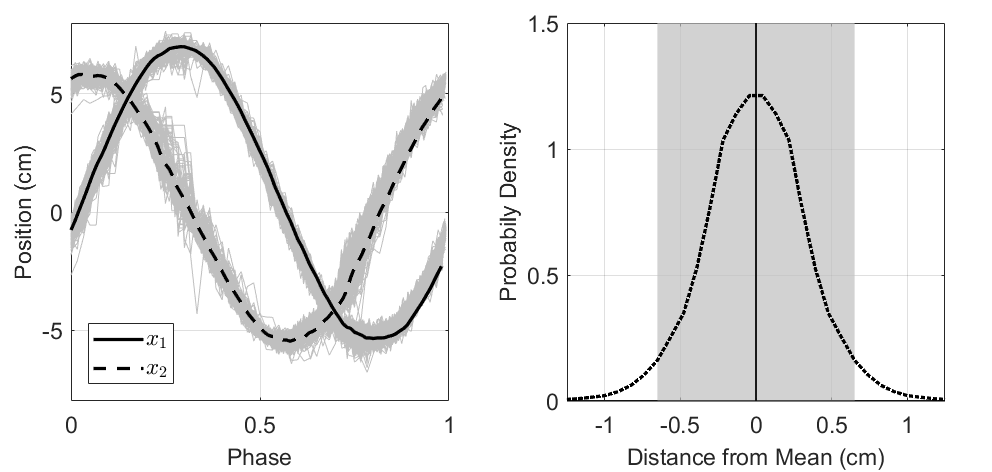
\includegraphics[width=\linewidth]{figures/noise.png}
    \caption{The left plot shows the average response of the system over a single period when the sinusoidal inputs of varying frequencies described by \eqref{eq:unoise} are applied. All of the particular responses are subimposed in light grey.
    The right plot shows the distribution of trajectories about the mean, with all distances within two standard deviations highlighted in grey. The width of the distribution illustrates how for the soft robot system identical inputs can produce outputs that vary by up to 2 cm.}
    \label{fig:noise}
\end{figure}

%% SUBS: DATA COLLECTION
\subsection{Data Collection and Model Identification}
\label{sec:datacollection}

% How data was collected
To construct a model, we ran the system through $16$ trials each lasting approximately $20$ minutes.
A randomized input was applied during each trial to generate a representative sampling of the system's behavior over its entire operating range.
To ensure randomization, a matrix, $\Upsilon \in [0,10]^{3\times 1000}$, of uniformly distributed random numbers between zero and ten was generated to be used as an input lookup table.
Each control input was smoothly varied between elements in consecutive columns of the table over a transition period $T_u$, with a time offset of $T_u / 3$ between each of the three control signals
\begin{align}
    u_i (t) &= \frac{(\Upsilon_{i,k+1} - \Upsilon_{i,k})}{T_u} \left( t + \frac{(i-1) T_u}{3} \right) + \Upsilon_{i,k}
    \label{eq:input}
\end{align}
where $k = \text{floor}\left( {t} / {T_u} \right)$ is the current index into the lookup table at time $t$. 
The transition period $T_u$ varied from $5$ seconds to $10$ seconds between trials.
After collection, the data was uniformly sampled with period $T_s = 0.1$ seconds.

% Models were build from this data
Two models were fit from the data: a Koopman model, and a linear state space model.
The linear state-space model provides a baseline for comparison and was identified from the same data as the Koopman model using the MATLAB System Identification Toolbox \cite{MATLAB:2017}.
This model is a four dimensional linear state-space model expressed in observer canonical form.
The Koopman model was identified via the method described in Section \ref{sec:sysid} on a set of $191,000$ snapshot pairs $\{ a[k] , b[k] \}$ that incorporate a single delay $d = 1$:
\begin{align}
    a[k] &= \begin{bmatrix} x[k]^\top & x[k-1]^\top & u[k-1]^\top \end{bmatrix}^\top \\
    b[k] &= \begin{bmatrix} \left( \phi_{T_s} (x[k]) + \sigma[k] \right)^\top & x[k]^\top & u[k]^\top \end{bmatrix}^\top,
\end{align}
and using the $N=330$ dimensional set of basis functions consisting of all monomials of maximum degree 4.
To find the sparsest acceptable matrix representation of the Koopman operator, equation \eqref{eq:lasso} was solved for ${ \lambda = 0,1,2, ... ,50 }$.
Predictions from the resulting models were evaluated against a subset of the training data, with the error quantified as the average Euclidean distance between the prediction and actual trajectory at each point, normalized by dividing by the average Euclidean distance between the actual trajectory and zero.
Fig.~\ref{fig:lasso} shows that as $\lambda$ increases so does this error, but the density of the $\hat{A}$ matrix of the lifted linear model decreases.
The model chosen is the one that minimizes both density and prediction error, which results in an $\hat{A}$ matrix with $70 \%$ of its entries equal to zero.

%% FIG: MODEL VS. WEIGHT OF L1 PENALTY (LASSO)
\begin{figure}
    \centering
    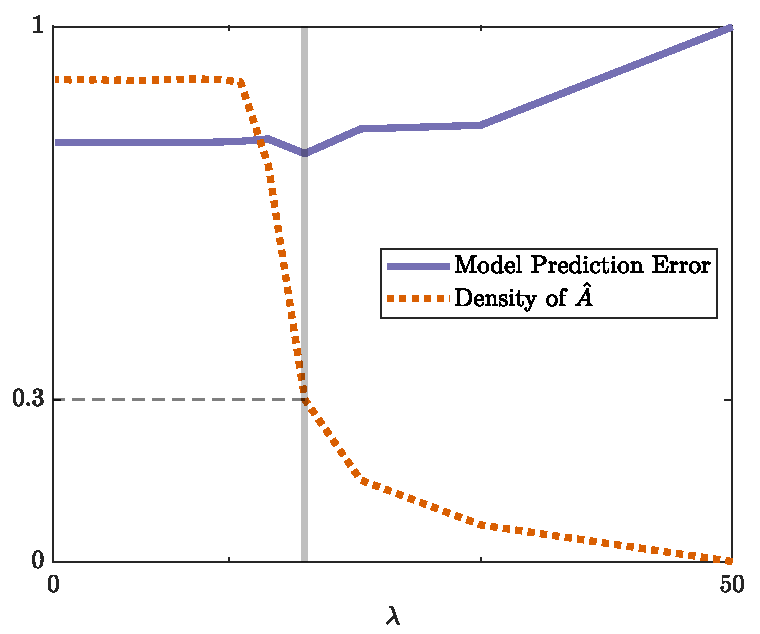
\includegraphics[width=\linewidth]{figures/lasso_v2.pdf}
    \caption{As $\lambda$ (the weight of the $L^1$ penalty term in \eqref{eq:lasso}) increases, the density of the lifted system matrix $\hat{A}$ decreases.
    The model generated by solving \eqref{eq:lasso} with the $\lambda$ valued designated by the vertical grey bar has lower error and a sparser $\hat{A}$ matrix than the least-squares solution to \eqref{eq:koopGamma}, which occurs at $\lambda = 0$. \Brent{I think it would be a good idea to include a label for the y-axis.  Perhaps just ``Matrix Density''. I suppose it's clear that matrix density is the inverse of sparsity and 1 means all non-zero. So we can leave out the units.} }
    \label{fig:lasso}
\end{figure}


%% SUBS: PREDICTOR COMPARISON
\subsection{Experiment 1: Model Prediction Comparison}
\label{sec:predict}

The accuracy of the predictions generated by each of the two models were evaluated by comparing them to the actual behavior of the system under the sinusoidal inputs defined in \eqref{eq:unoise}.
The model responses were simulated over a time horizon of $2.5$ seconds given the same initial condition and input as the real system.
The results of this comparison are summarized by Fig. \ref{fig:predict} and Table \ref{tab:predict}. 
They illustrate that the Koopman model predictions are more accurate over the time horizon.
\Ram{probably want to describe performance in relation to stochastic behavior.}

%% FIGURE: Linear vs. Koopman model predictions
\begin{figure}
    \centering
    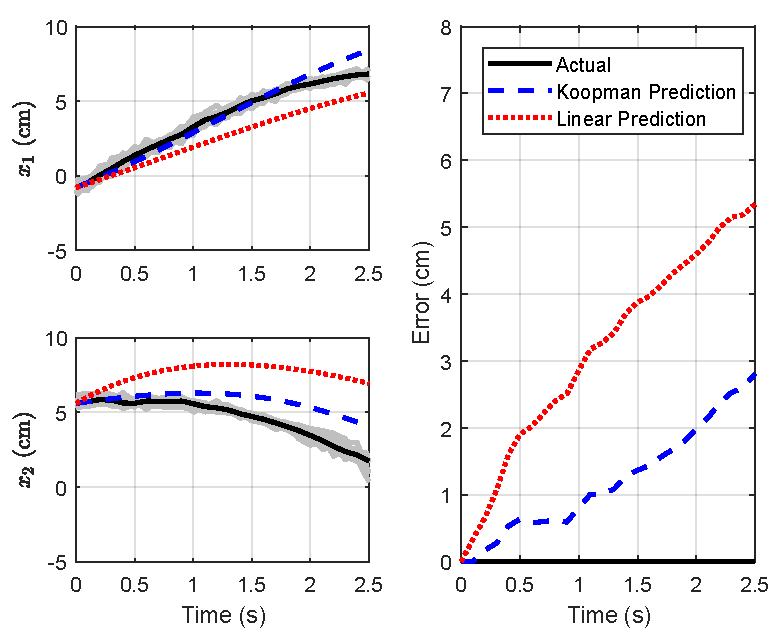
\includegraphics[width=\linewidth]{figures/predictionComparison_v3.pdf}
    \caption{The average actual response and the model predictions for the robot over a 2.5 second horizon with the sinusoidal inputs described in \eqref{eq:unoise} with period $T = 10$ seconds applied. The left side shows the laser dot position projected into each coordinate separately. The error displayed on the right plot is defined as the Euclidean distance between the predicted laser dot position and the average actual position at each point in time. \Brent{If you need to save space, I think you can remove the Error plot on the right.  The errors are already visible in the plots on the left, even if they are in state space variables.  Also, the table of Euclidean error is also available.  }}
    \label{fig:predict}
\end{figure}

%% TABLE: Prediction Comparison
\begin{table}
    \rowcolors{2}{white}{gray!25}
    \setlength\tabcolsep{5pt} % default value: 6pt
    \centering
    \caption{Average Prediction Error Over 2.5 second Horizon (cm)}
    \begin{tabular}{|c|c|c|c|c|c|c|c|c|}
        \hline
        \rowcolor{white} 
        & \multicolumn{7}{c |}{\textbf{Period of Sinusoidal Inputs (seconds)}} & \\
        \cline{2-4} \rowcolor{white}
        \multirow{-2}{*}{\textbf{Model}} & 6 & 7 & 8 & 9 & 10 & 11 & 12 &\multirow{-2}{*}{\textbf{Avg.}} \\
        \hline
        % RESULTS FOR ROBOT A
        Koopman &  2.21  &  2.78 &  1.35  &  1.53  &  1.21 & 0.66 & 1.41 & 1.59 \\
        Linear S.S.  &  4.64  &  4.54  &  3.94 &  3.56  & 3.15 & 2.72 & 2.83 & 3.63 \\
        % Ham.-Weiner &  7.0  &  4.5  &  6.9  &  3.0  &  2.3  &  3.1 & 4.5 & 2.0 \\
        % \multirow{-5}{*}{\cellcolor{white} \rotatebox[origin=c]{90}{\textbf{Robot A}}}
        % NLARX       &  5.0  &  3.0 &  12.0  &  3.8  &  2.1  &  2.8 & 4.8 & 3.7 \\
        \hline
        % % RESULTS FOR ROBOT B
        % \cellcolor{white} & Koopman & & & & & & & & \\
        % \cellcolor{white} & Neural Net & & & & & & & & \\
        % \cellcolor{white} & State Space & & & & & & & & \\
        % \cellcolor{white} & Ham.-Weiner & & & & & & & & \\
        % \multirow{-5}{*}{\cellcolor{white} \rotatebox[origin=c]{90}{\textbf{Robot B}}}
        % & NLARX & & & & & & & & \\
        % \hline
    \end{tabular}
    \label{tab:predict}
\end{table}





%% SUBS: Description of the controllers and tracing task
\subsection{Experiment 2: Model-Based Control Comparison}
\label{sec:mpcexp}
% \Dan{Lot's of imprecise explanations in this section}

%% Description of compared controllers
The two identified models were each used to build a model predictive controller which solves an optimization problem in the form of \eqref{eq:mpc} at each time step.
We refer to the two controllers by the abbreviations K-MPC for the one based on the Koopman model, and L-MPC for the one based on the linear state-space model. 
%Or: We use the abbreviation K-MPC to refer to the controller based on the Koopman model and L-MPC for the controller based on the linear state-space model.  
Both model predictive controllers run in closed-loop at $10$ Hz, feature an MPC horizon of 2.5 seconds ($N_h = 25$), and a cost function that penalizes deviations from a reference trajectory $r[k]$ over the horizon with both a running and terminal cost:
\begin{align}
    \text{Cost} &= 100 \left( y[N_h] - r[N_h] \right)^2 + \sum_{i=0}^{N_h - 1} 0.1 \left( y[i] - r[i] \right)^2
\end{align}
In the K-MPC case, $y[i] = C z[i]$, where $C$ is defined as in \eqref{eq:C}.
In the L-MPC case, $y[i] = C_L x_L[i]$ where $x_L$ is the four dimensional system state and $C_L$ is the projection matrix that isolates the states describing the current laser dot coordinates. 

% The optimization problem for each controller also featured a convex constraint to limit the rate at which the control inputs could change over time... 

% task
The performance of the controllers was assessed with respect to a set of two trajectory following tasks.
Each task was to follow a reference trajectory as it traced out the following shapes over a certain amount of time:
\begin{enumerate}
    \item Pacman (90 seconds)
    \item Star (180 seconds)
    \item Block $\Sigma$ (300 seconds)
\end{enumerate}
The error for each trial was quantified as the Cartesian distance from the reference trajectory at each time step over the length of the trial.

The performances of the K-MPC and L-MPC controllers at Tasks 1, 2, and 3 are shown visually in Fig. \ref{fig:results}, and the error is quantified in Table \ref{tab:RMSE}.
In both tasks the K-MPC controller \Brent{achieved better performance} \sout{performed best}, exhibiting an average tracking error of 1.26~cm compared to the L-MPC controller's average error of 2.45~cm.
This amounts to an average error roughly $25\%$ larger than than the maximum magnitude of observed noise (see Fig. \ref{fig:noise})
% The magnitude of this error was larger than the maximum magnitude of observed noise (see Fig. \ref{fig:noise}), but only by about one quarter of a centimeter, or $1 \%$ of the total range of motion observed. 



%% FIGURE: Visual results
\begin{figure*}
    \centering
    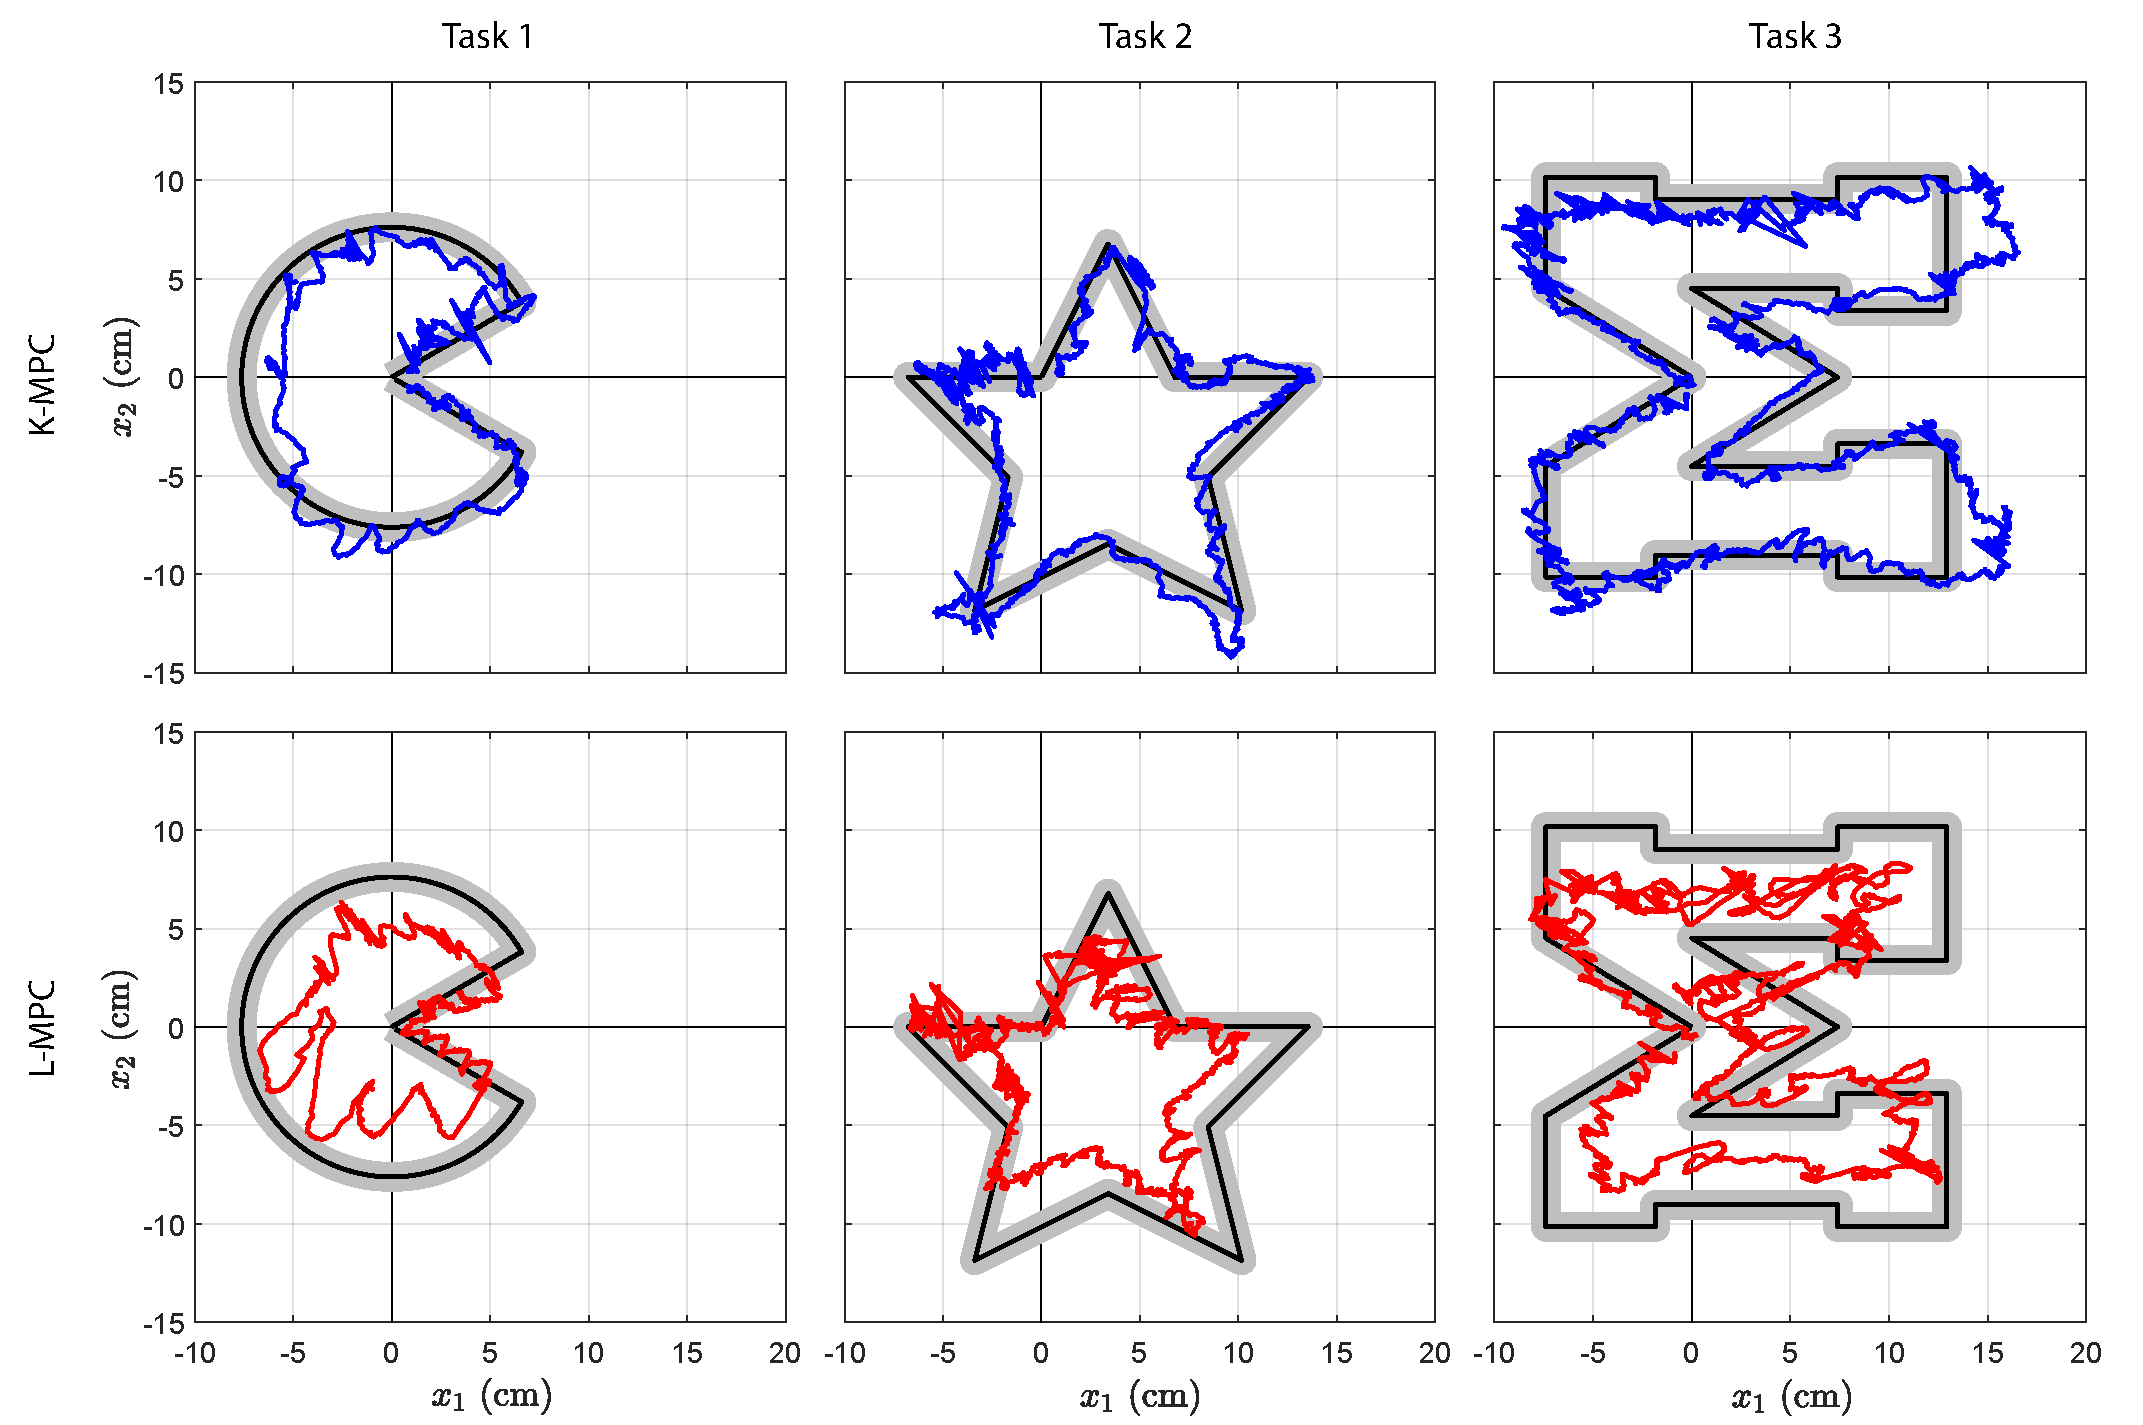
\includegraphics[width=\linewidth]{figures/results_edited_wblue.pdf}
    \caption{The results of the K-MPC controller (row 1, blue) and the L-MPC controller (row 2, red) in performing trajectory following tasks 1-3. The reference trajectory for each task is subimposed in black as well as a grey buffer with width equal to two standard deviations of the noise probability density shown in Fig. \ref{fig:noise}.}
    \label{fig:results}
\end{figure*}

%% TABLE: RMSE results table
\begin{table}
    \rowcolors{2}{white}{gray!25}
    \setlength\tabcolsep{5pt} % default value: 6pt
    \centering
    \caption{Average Error in Trajectory Following Tasks (cm)}
    \begin{tabular}{|c|c|c|c|c|c|}
        \hline
        \rowcolor{white} 
        & \multicolumn{3}{c |}{\textbf{Task}} & & \textbf{Std.} \\
        \cline{2-4} \rowcolor{white}
        \multirow{-2}{*}{\textbf{Controller}} & $1$ & $2$ & $3$ & \multirow{-2}{*}{\textbf{Avg.}} & \textbf{Dev.} \\
        \hline
        % RESULTS FOR ROBOT A
        K-MPC &  1.25  &  1.19 &  1.34  &  1.26  &  0.07  \\
        L-MPC  &  2.21  &  2.34  &  2.73 &  2.45  &  0.31   \\
        % Ham.-Weiner &  7.0  &  4.5  &  6.9  &  3.0  &  2.3  &  3.1 & 4.5 & 2.0 \\
        % \multirow{-5}{*}{\cellcolor{white} \rotatebox[origin=c]{90}{\textbf{Robot A}}}
        % NLARX       &  5.0  &  3.0 &  12.0  &  3.8  &  2.1  &  2.8 & 4.8 & 3.7 \\
        \hline
        % % RESULTS FOR ROBOT B
        % \cellcolor{white} & Koopman & & & & & & & & \\
        % \cellcolor{white} & Neural Net & & & & & & & & \\
        % \cellcolor{white} & State Space & & & & & & & & \\
        % \cellcolor{white} & Ham.-Weiner & & & & & & & & \\
        % \multirow{-5}{*}{\cellcolor{white} \rotatebox[origin=c]{90}{\textbf{Robot B}}}
        % & NLARX & & & & & & & & \\
        % \hline
    \end{tabular}
    \label{tab:RMSE}
\end{table}
\section{Conclusion}
\label{sec:conclusion}

% Reiteration of contribution
In this work, a data-driven modeling and control method based on Koopman operator theory was successfully applied to a soft robot.
The Koopman-based MPC controller was shown to be capable of commanding a soft robot to follow a reference trajectory better than an MPC controller based on another linear data-driven model.
% Reiterarion of why important for soft robotics
By making explicit control-oriented models of soft robots easier to construct, this method enables the rapid development of new control strategies and applications.

% Current shortcomings that should be addressed in future work (more dynamics excitement, higher dimensional systems)
While these preliminary results are promising, further work is needed to make such methods feasible for higher dimensional robotic systems.
Toward that end, this work introduced a method for promoting sparsity in matrix representations of the Koopman model.
Additional work will explore strategies for further promoting sparsity, choosing the most effective basis of observables, and building models that can account for external loading and contact forces.





% \Dan{For now this is just a list of talking points}
% Discussion of results:
% The model predictive controller using the the Koopman model outperformed the other controllers in a variety of trajectory following tasks.

% Sources of Error:
% -Model inaccuracies due to insufficient data.
% -Model inaccuracies due to Koopman truncation.
% -Poor performance of electronic pressure regulators.
% -Limited accuracy of camera based laser tracking system.

% Current Shortcomings of Method:
% -Curse of dimensionality, but sparsity could help (cite that paper)
% -Does not generalize outside of observed data, could be solved by switching controllers/hybrid models.

% Take Aways:
% -Has potential to revolutionize soft robot control by providing much more control friendly representation of dynamics.
% -Soft robots are well suited for a data-driven method because they can be observed safely under randomized control inputs.
% -This is the first time this method has been shown to be effective for controlling a real soft robotic system.

% \section*{Acknowledgments}

%% Use plainnat to work nicely with natbib. 

\bibliographystyle{plainnat}
\bibliography{references}

\end{document}
